\documentclass[11pt,a4paper]{article}
\usepackage{graphicx}
\usepackage{listings}
\usepackage{color}
\usepackage{url}
\usepackage{hyperref}
\hypersetup{
    colorlinks=true,
    linkcolor=black,
    filecolor=black,      
    urlcolor=cyan,
    pdftitle={Overleaf Example},
    pdfpagemode=FullScreen,
    }
\usepackage[nottoc,numbib]{tocbibind}

\definecolor{dkgreen}{rgb}{0,0.6,0}
\definecolor{gray}{rgb}{0.5,0.5,0.5}
\definecolor{mauve}{rgb}{0.58,0,0.82}

\lstset{frame=tb,
  language=Java,
  aboveskip=3mm,
  belowskip=3mm,
  showstringspaces=false,
  columns=flexible,
  basicstyle={\small\ttfamily},
  numbers=none,
  numberstyle=\tiny\color{gray},
  keywordstyle=\color{blue},
  commentstyle=\color{dkgreen},
  stringstyle=\color{mauve},
  breaklines=true,
  breakatwhitespace=true,
  tabsize=3
}


\graphicspath{ {./images/} }
\title{Sentiment Analysis of Tweets using multiple Algorithms \\[0.5em] \large{Project Report for "Data Mining" \\[0.5em]} }

\author{David Riemer, Olivia Saukonoja}

\date{December 2023}



\begin{document}
\maketitle


\newpage
\begin{abstract}
In this Project Report we will explain in detail the process of our Python Project, in which we use multiple algorithms discussed in class to find relationships between words used in tweets. The Dataset provided by the kaggle competition "Twitter sentiment analysis" includes 100000 tweets as Training Data, with their given Sentiment. 1 as a representation for a positive tweet and 0 for a negative one.
This project utilizes various algorithms, including k-means clustering, Hashing, Dimension Reduction by Singular Vector Decomposition, and A-priori. By applying these algorithms, we aim to gain insights into patterns and connections within the datasets' content. 
This analysis will contribute to a better understanding of the relationships between words and their context in the realm of social media data. 
Throughout this report, we will delve into the methodology, results, and implications of the algorithms, highlighting the steps necessary for a successful interpretation of the results and also which obstacles had to be overcome on the way but also what room for improvement is available.
In the end we will build a Logistic Regression-model in order to classify other tweets to their respective Sentiment value and give a conclusion about our Project.
\end{abstract}
\newpage
\tableofcontents
\newpage
\section{Introduction}
The importance of Natural Language Processing (NLP) has grown significantly due to the overabundance of data on the internet. With the vast amount of text-based information available online, it has become increasingly challenging for humans to manually process and extract meaningful insights from this data. NLP techniques, such as text classification, sentiment analysis, and named entity recognition, enable us to automate the analysis and understanding of large volumes of text data. 
One of the motivations of our project is the fact, that tweets provide a short form of information singlehandedly, however in bulk they reveal hidden trends and connections between various users. 
In the first section of this report we will explain the methods used in our data mining process, which include Word2Vec, Dimension Reduction, k-means Clustering, A-priori as well as Logistic Regression, in order to build a solid fundation of knowledge, for the purpose of comprehending the following chapters better. This is also the section where we describe the given data. After that, we will present the results from our algorithms to provide more detailed information about the outcome of our project.
In the context of our projext our main source of information was the book \emph{Mining of massive data sets} written by Anand Rajaraman, Jure Leskovec, and Jeffrey D. Ullman \cite{leskovec2020mining}.
\section{Methods}
\subsection{Architecture and Environment}
For our project enviroment we opted to use Visual Studio Code 1.84 on Windows 11. In order to be able to work better with our large dataset we decided to include Pyspark, which ran locally on my RazerBook 13. On top of that for some of the visualization we also used Knime with its respective JavaScript extension.
\subsection{The data}
The dataset utilized for this project can be accessed on \href{https://www.kaggle.com/competitions/twitter-sentiment-analysis2}{this Kaggle competition} 
It consists of a CSV file with the following columns:
\begin{itemize}
\item ItemID: This column serves as the primary key, assigning a unique number to each tweet.
\item Sentiment: This column indicates the sentiment of each tweet. A value of 0 denotes a negative sentiment, while a value of 1 signifies a positive sentiment.
\item SentimentText: The content of the tweets is contained within this column.
\end{itemize}
The dataset consists of a total of 100,000 tweets. After analyzing the data, we aimed to describe some basic properties of the dataset. Our research concluded that there are 56,462 positive tweets and 43,538 negative tweets (figure \ref{sentiment}). The tweet with the highest word count consisted of 70 words, while the shortest tweet contained only 1 word. On average, users tend to use 15 words per tweet. This average applies to 4,167 tweets. Additionally, the most frequently used word (after applying our pipeline) is "good", and 72,796 people tweeted 20 words or less.
\begin{figure}[h]
\caption{Basic Visulization of the dataset}
\label{sentiment}
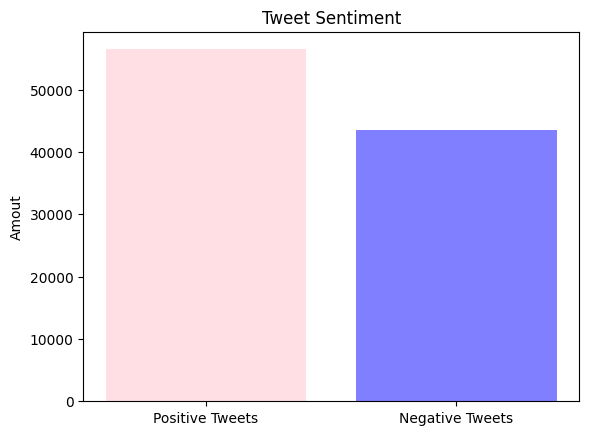
\includegraphics[scale=0.38]{output}
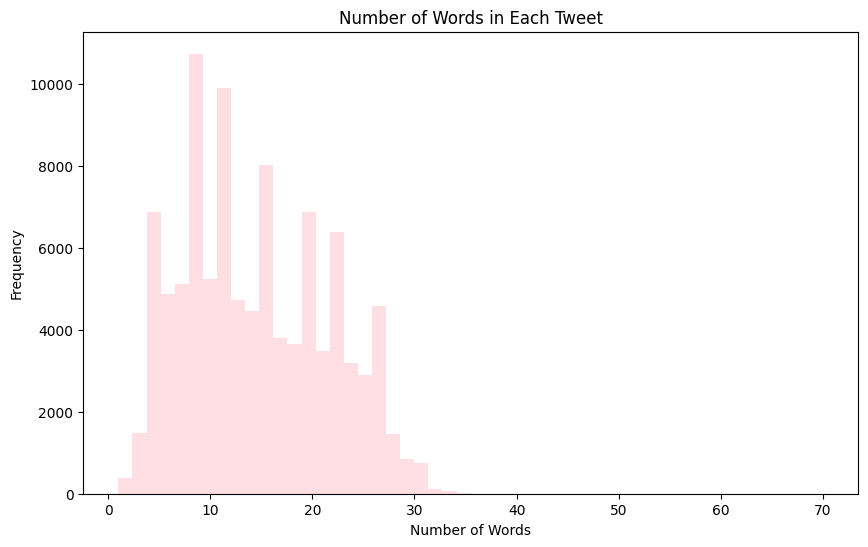
\includegraphics[scale=0.3]{numberofwords}
\centering
\end{figure}
\subsection{Preprocessing of the data}
The first step of our the pipeline is tokenization, which is the process of splitting the text into individual words or tokens. This is done using the "RegexTokenizer". The "inputCol" parameter is set to "SentimentText", which is the column in the DataFrame that contains the text to be tokenized.. The "pattern" parameter of the Tokenizer is set to "\\W", which means any non-word character is considered a delimiter. The second step in the pipeline is "stop words removal". Stop words are common words that do not carry much meaningful information and are often removed in text mining tasks. The "StopWordsRemover" class is used for this purpose. In order to eliminate all necessary stop words we imported the english stopwords corpus fromm nltk.corpus and added some custom stop words, like websites or hyperlinks. The third step in the pipeline is feature extraction. The "HashingTF" class converts all the words leftover after removing the stop words into numerical feature vectors.
To run these steps sequentially and have them contained in one object, we created a variable called pipeline. It includes all the steps mentioned above. This also makes it easier to rerun the pipeline if necessary. As mentioned in the introduction, our goal is to gain an overview of the extensive dataset provided.We want to create a Logistic Regression Model that can predict the sentiment of a tweet with at least 70\% accuracy. Additionally, we would like to understand the relationships between words used in tweets, such as identifying the words most likely used in the context of a tweet that also contains the word "happy."
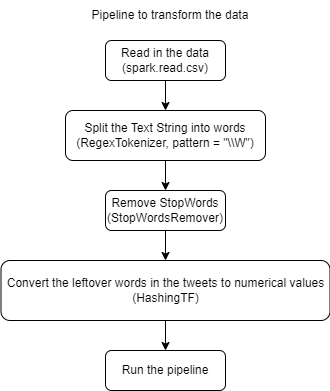
\includegraphics[scale = 0.5]{pipeline}
\subsection{Clustering the data with the help of Word2Vec}
In order to get to a point of clustring the words in a way that makes sense, we decided to train a Word2Vec model. Word 2Vec is a standard method of generating word embeddings: This is a process of each word being mapped to an vector in a high dimensional space. By mapping words to continuous vector representations, word embeddings enable NLP models to understand the similarity, analogy, and relatedness between different words\cite{cluster}\cite{gensimword2vec}. We decided on our vector to be of the dimension 2000.  
\begin{lstlisting}
w2vModel = Word2Vec(sentences=sentences, vector_size=2000, workers=1, seed=1337)
w2vModel.save("word2vec.model")
\end{lstlisting}
After creating the model, we then used it to find out which words are most often used with the most common emotions expressed in tweets:
\begin{lstlisting}
listHappy=w2vModel.wv.most_similar("happy")
listsad=w2vModel.wv.most_similar("sad")
listgood=w2vModel.wv.most_similar("good")
listbad=w2vModel.wv.most_similar("bad")
\end{lstlisting}
\begin{figure}[h]
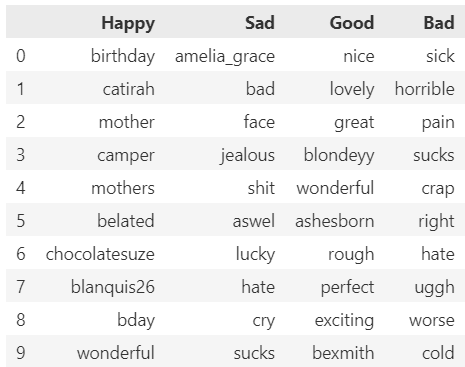
\includegraphics[scale=0.6]{emotionwords}
\centering
\end{figure}
Our goal is to have words with similar context occupy close spatial positions when we end up plotting our data. 
\subsubsection{Dimensionreduction suing Singular Vector Decomposition (SVD)}
After generating the 2000-dimensional vector representation for each word, the next step is to apply Singular Value Decomposition (SVD) to these vectors. This will allow us to plot the data points (words) on a 2-dimensional coordinate system in the subsequent step. This is acomplished by importing svd from scipy.linalg.
\begin{lstlisting}
from scipy.linalg import svd
from numpy import zeros, diag
\end{lstlisting}
We also just want to look at the 750 "most important" words in our dataset so we end up with a \(750 \times 2000\) matrix, in which each row is a representation of one word and the columns represent one of the features of the word. After creating our \(U, \sigma,~and~V^T \) matrices and reducing the dimensions to only 2 by selecting only the two largest singular values and their corresponding singular vectors from these 3 matrices and multiplying them together, we create a new Matrix B. \cite{banerjee2014linear}
\begin{lstlisting}
U, s, VT = svd(vectors750, full_matrices=False)
Sigma = zeros((vectors750.shape[0], vectors750.shape[1]))
Sigma[:vectors750.shape[0], :vectors750.shape[0]] = diag(s)
n_elements = 2
Sigma = Sigma[:, :n_elements]
VT = VT[:n_elements, :]
#reconstruct
B = U.dot(Sigma.dot(VT))
\end{lstlisting}
\subsubsection{Using k-means to cluster the data and visualize}
Now we can plot the data in a 2-dimensional space in which words most often used together are close to one another in the euclidean space. We use the k-means package provided by sklearn.cluster and devide the points in 20 cluster and also end up plotting the respective centroid of each cluster to visualize the data better. In the result,we observed that words describing days of the week and points in time belong to one cluster, as well as words associated with positive emotions. However, there is a lot of noise in the middle of the figure, mainly because many words can be used in various contexts.
\begin{figure}[htp]
\centering
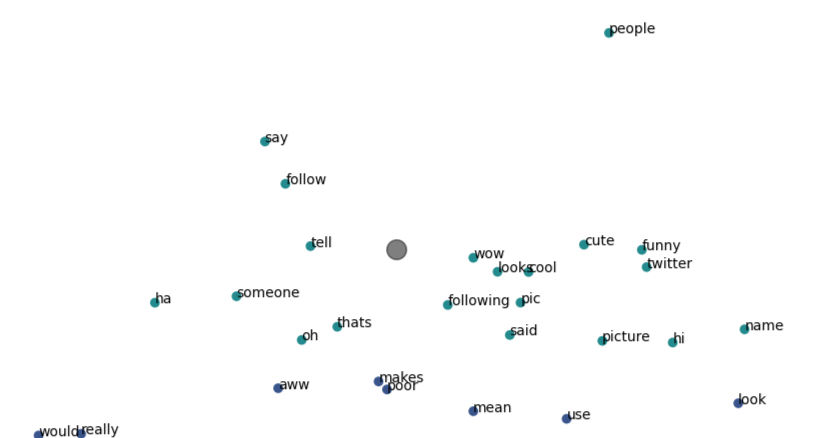
\includegraphics[width=.3\textwidth]{kmeanspositive}\hfill
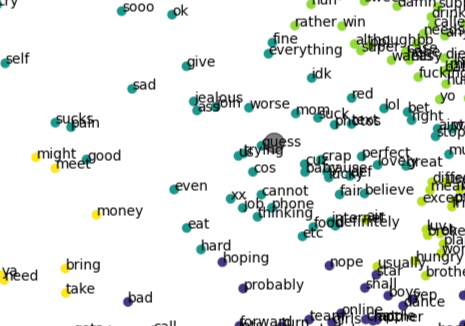
\includegraphics[width=.3\textwidth]{kmeansnegative}\hfill
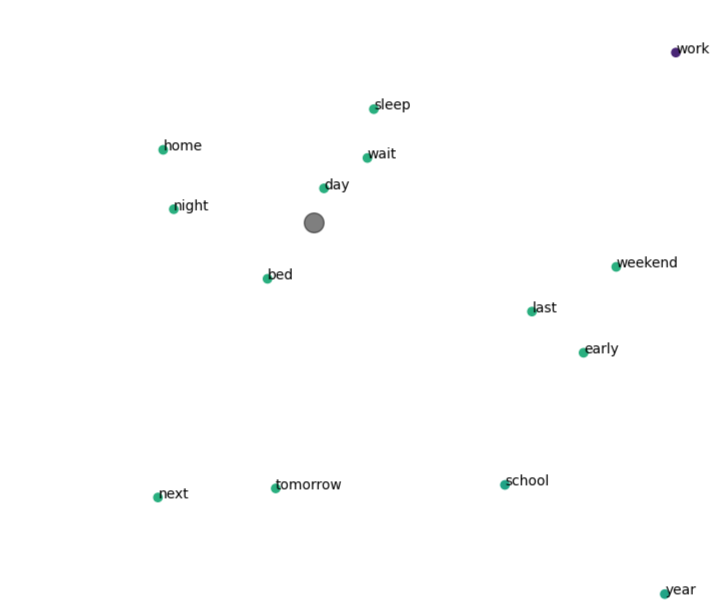
\includegraphics[width=.3\textwidth]{kmeansdates}
\caption{On the left: positive emotions(wow, cool, cute, funny) \\ Middle: negative emotions(jealous, sad, worse, cannot)\\ Right: Timestamps used in the context of sleep (bed, night, slep, tomorrow)}
\label{fig:kmeansresult}
\end{figure}
\subsection{A-priori to find words most often used together}
Next, we used a simple implementation of the Apriori algorithm in order to find words that are often used together. This time only the number of occurences of a word in a tweet is examined. We chose the support threshold to be 0.002 and our minimum confidence to be 0.1.
We also divided our preprocessed dataset into two separate dataframes. One dataframe includes only positive tweets, while the other includes only negative tweets.
The top 5 most frequently used words in positive tweets were "good," "thanks," "love," "lol," and "like." In negative tweets, the most common words were "get," "like," "know," "sorry," and "go." The most frequently occurring tuple in positive tweets was [morning, good], and in negative tweets, it was [could, wish].
\subsection{Logistic Regression Model}
In the final step of our project, we developed a Logistic Regression Model to classify tweets based on their sentiment.
To begin, we randomly divided the data into 80\% training data and 20\% test data. When creating the Logistic Regression Model, we set a maximum of 1000 iterations to ensure convergence even if the gradient descent steps become "stuck". Additionally, we included a regularization parameter to prevent overfitting on the training data.
Regarding the features used to train the model, we employed the features from the hashingTF in our initial pipeline.
\newpage
\begin{lstlisting}
Split training and Testing
split_data=train.randomSplit([0.8,0.2])
trainSplit=split_data[0]
testSplit=split_data[1]
trainSplit = pipeline.transform(trainSplit).select("Sentiment", "filtered", "features")
testSplit = pipeline.transform(testSplit).select("Sentiment", "filtered", "features")
lr = LogisticRegression(labelCol = 'Sentiment', featuresCol='features', maxIter=1000, regParam=0.01)
lrModel = lr.fit(trainSplit)
print("Done")
\end{lstlisting}

\section{Results and Conclusion}
In this project, we aimed to find relationships between words used in 100,000 tweets. The used algorithms Word2Vec, Dimension Reduction, k-means clustering, A-priori and Logistic Regression were able to find different kinds of relationships between words.
First, data was clustered using Word2Vec model to vectors in a 2000-dimensional space. Then the model was used to find out words in the context of common emotions, generally expressed in tweets. These emotions were “happy”, “sad”, “good” and “bad”, and the words with similar context were represented in a table that includes one column for each emotion.
After that, Dimension Reduction by Singular Vector Decomposition was applied to these vectors. This resulted the data points being plotted on a 2-dimensional space to a 750 x 2000 matrix. The rows of the matrix were representations of words, and the columns were the features of the word. We applied SVD to reduce the dimensionality of the word vectors while preserving the semantic relationships, enabling us to visualize the word embeddings in a 2-dimensional space.
Then k-means was used to cluster the data into 20 clusters based on which words are most often used together. The centroids of each cluster were also plotted to visualize the data. Through this visualization, we observed that words most often used together were closer to each other in the Euclidean space, indicating their semantic similarity and contextual usage.
Next, A-priori algorithm was used to find words that often occur together. The positive and negative tweets were analyzed separately. The result of this was that five most frequently used words in positive tweets were “good”, “thanks”, “love”, “lol” and “like”. In negative tweets, the most common words were “get”, “like”, “know”, “sorry”, and “go”. 
The most common tuple in positive tweets was [morning, good] and in negative tweets [could, wish]. 
Finally, Logistic Regression Model was used to classify the tweets based on their sentiment in 1000 iterations. Our goal was to create a model of 70\% acuraccy, which we succeded in achieving.
In conclusion, the algorithms were applicable to mining information from tweets. They were also able to successfully find different kinds of patterns. Finally, they were able to reveal connections between words and extract meaningful information from the data.
\subsection{Further improvements}
Although these observations initially seem logical, our results still present conflicting findings. For instance, it seems contradictory that the word "good" is one of the most frequently used words in negative tweets as well. This discrepancy could be attributed to various factors: First of all it is difficult to cleanse all the tweets of both sentiments to just their important words. We tried our best to remove stopwords, but some words can be used in a rich amount of contexts, particularly in both sentiments. We made an effort to remove stop words, adding custom ones as well, but some words can be used in various contexts, especially in both positive and negative sentiments. In future studies, we believe that implementing more advanced preprocessing techniques could yield improved results, not only in classification but also in generating more intuitive visualizations on the graph. Another way to improve classification could be by implementing a third "neutral" sentiment. Negative tweets would have a sentiment of -1, neutral tweets would have a sentiment of 0, and positive tweets would have a sentiment of 1\cite{twitter-sentiment-analysis2}. This approach could help in removing some of the ambiguities in words, as identified in our apriori analysis.
\bibliographystyle{unsrt}
\bibliography{bibtex}







\end{document}
